\documentclass[12pt,a4paper]{article}

\usepackage[utf8]{inputenc}
\usepackage[T1]{fontenc}
\usepackage{lmodern}
\usepackage[margin=1in]{geometry}
\usepackage{amsmath,amssymb}
\usepackage{graphicx}
\usepackage{booktabs}
\usepackage{tabularx}
\usepackage{array}
\usepackage{xcolor}
% float must precede hyperref, or every [H] float gets a duplicate PDF anchor.
\usepackage{float}
\usepackage{hyperref}
\usepackage{cleveref}
\usepackage{natbib}
\usepackage{setspace}
\usepackage{enumitem}

\hypersetup{pdftitle={How Much Does the Model Move the Allowance? Equally Accurate Default Models and the CECL Reserve},
  pdfauthor={Akram Khan},
  pdfsubject={Dispersion of lifetime expected credit losses across equally accurate loan-level default models, measured on Freddie Mac data},
  pdfkeywords={CECL, ASC 326, IFRS 9, allowance for credit losses, model risk, model multiplicity, Rashomon set, mortgage default, SAB 119},
  colorlinks=true, linkcolor=blue!70!black, citecolor=green!50!black, urlcolor=blue!70!black}
\onehalfspacing
\emergencystretch=3em

% Generated by code/09_paper.py. Do not edit.
\makeatletter
\newcommand{\num}[1]{\@ifundefined{num@#1}{\errmessage{Undefined number: #1}}{\@nameuse{num@#1}}}
\@namedef{num@H1.n}{13}
\@namedef{num@H1.verdict}{holds}
\@namedef{num@H2.n}{21}
\@namedef{num@H2.verdict}{holds}
\@namedef{num@H3.median}{56}
\@namedef{num@H3.rel2006}{37}
\@namedef{num@H3.rel2007}{46}
\@namedef{num@H3.verdict}{fails}
\@namedef{num@H4.n}{12}
\@namedef{num@H4.verdict}{holds}
\@namedef{num@H5.above}{4}
\@namedef{num@H5.below}{8}
\@namedef{num@H5.first}{2005}
\@namedef{num@H5.inside}{1}
\@namedef{num@H5.inside25}{2}
\@namedef{num@H5.last}{2017}
\@namedef{num@H5.n_elig}{13}
\@namedef{num@H5.verdict}{holds}
\@namedef{num@H6.n}{17}
\@namedef{num@H6.verdict}{holds}
\@namedef{num@const.hours}{11}
\@namedef{num@const.n_boot}{1{,}000}
\@namedef{num@const.n_dates}{21}
\@namedef{num@const.n_features}{20}
\@namedef{num@const.n_models}{65}
\@namedef{num@const.n_port}{200{,}000}
\@namedef{num@data.act_2020}{46}
\@namedef{num@data.active_2025}{13.1}
\@namedef{num@data.ce_2009}{67}
\@namedef{num@data.ce_2020}{3.3}
\@namedef{num@data.dr_2020}{2.04}
\@namedef{num@data.dr_peak_gfc}{1.88}
\@namedef{num@data.dr_peak_gfc_year}{2010}
\@namedef{num@data.excl_hpi}{74{,}879}
\@namedef{num@data.excl_ltv}{1{,}853}
\@namedef{num@data.jud.higher}{110}
\@namedef{num@data.jud.n}{119}
\@namedef{num@data.kept}{49{,}406{,}273}
\@namedef{num@data.loan_years}{221.4}
\@namedef{num@data.orig_rows}{49{,}483{,}298}
\@namedef{num@data.panel_loans}{47.1}
\@namedef{num@data.perf_rows}{2.92}
\@namedef{num@data.po_2020}{45}
\@namedef{num@data.quarters}{110}
\@namedef{num@dec.late.maxdev}{28}
\@namedef{num@dec.lgd.max}{2.9}
\@namedef{num@dec.lgd.min}{1.8}
\@namedef{num@dec.lgd19.max}{3.7}
\@namedef{num@dec.lgd19.min}{2.3}
\@namedef{num@dec.lgd19.over2006}{18}
\@namedef{num@dec.lgd19.short.max}{23}
\@namedef{num@dec.path.max}{5}
\@namedef{num@dec.path.min}{1.3}
\@namedef{num@dec.pre.below_lb}{3}
\@namedef{num@dec.pre.n}{4}
\@namedef{num@dq.2009.cur}{0.64}
\@namedef{num@dq.2009.d30}{23.1}
\@namedef{num@dq.2009.d90}{76.2}
\@namedef{num@dq.share.max}{3.6}
\@namedef{num@dq.share.max_year}{2009}
\@namedef{num@dq.share.min}{0.8}
\@namedef{num@mac.hpi2005}{8.9}
\@namedef{num@mac.hpi2006}{4.9}
\@namedef{num@p2.below_median}{14}
\@namedef{num@p2.boot.rel}{52}
\@namedef{num@p2.boot_gt_rsm}{8}
\@namedef{num@p2.disj.lfl}{32}
\@namedef{num@p2.disj.rsm}{61}
\@namedef{num@p2.h4.lgbm}{38}
\@namedef{num@p2.h4.mono}{42}
\@namedef{num@p2.h4.n}{12}
\@namedef{num@p2.h4.smaller}{15}
\@namedef{num@p2.in_refit}{1}
\@namedef{num@p2.in_rsm}{0}
\@namedef{num@p2.median_gap}{2}
\@namedef{num@p2.paired1.single}{7}
\@namedef{num@p2.pos.median}{23}
\@namedef{num@p2.rho_rsm.median}{0.02}
\@namedef{num@p2.rho_rsm.pos}{12}
\@namedef{num@p2.rho_set.median}{0.30}
\@namedef{num@p2.rho_set.pos}{17}
\@namedef{num@pd.late.max}{0.82}
\@namedef{num@pd.late.min}{0.54}
\@namedef{num@pd.pre.max}{1.37}
\@namedef{num@pd.pre.min}{0.75}
\@namedef{num@ph.H1.n}{8}
\@namedef{num@ph.H1.ratio}{0.84}
\@namedef{num@ph.H1.refitmore}{13}
\@namedef{num@ph.H6.fliprefit}{27.5}
\@namedef{num@ph.H6.flipset}{18.4}
\@namedef{num@ph.frac.min}{2.8}
\@namedef{num@ph.frac.min_year}{2025}
\@namedef{num@ph.lfl.rel.median}{49}
\@namedef{num@ph.paired2.rel}{17}
\@namedef{num@ph.paired2.size}{7}
\@namedef{num@ph.rq.above}{18}
\@namedef{num@ph.rq.bias}{11}
\@namedef{num@ph.rq.gap}{0.8}
\@namedef{num@ph.rq.gt1}{111}
\@namedef{num@ph.rq.gt1.share}{26}
\@namedef{num@ph.rq.total}{420}
\@namedef{num@ph.rs.bias}{6}
\@namedef{num@ph.rs.bias.pos}{19}
\@namedef{num@ph.rs.disj.first}{2018}
\@namedef{num@ph.rs.disj.n}{8}
\@namedef{num@ph.rs.disj.refitmore}{6}
\@namedef{num@ph.rs.flip}{27.1}
\@namedef{num@ph.rs.flipmore}{4}
\@namedef{num@ph.rs.gap}{0.14}
\@namedef{num@ph.rs.mut.max}{81}
\@namedef{num@ph.rs.mut.max_year}{2005}
\@namedef{num@ph.rs.n}{12}
\@namedef{num@ph.rs.ov.max}{22}
\@namedef{num@ph.rs.ov.max_year}{2005}
\@namedef{num@ph.rs.ratio}{1.09}
\@namedef{num@ph.rs.rel.median}{49}
\@namedef{num@ph.rs.w95}{14}
\@namedef{num@res.auc.max}{0.910}
\@namedef{num@res.auc.min}{0.869}
\@namedef{num@res.best_rate.max}{2.39}
\@namedef{num@res.best_rate.max_year}{2011}
\@namedef{num@res.best_rate.min}{0.06}
\@namedef{num@res.both.rel.median}{57}
\@namedef{num@res.fam.lgbm.median}{38}
\@namedef{num@res.fam.mono.median}{42}
\@namedef{num@res.flip.median}{27.1}
\@namedef{num@res.flip_refit.median}{27.5}
\@namedef{num@res.loan.ratio.max}{7.9}
\@namedef{num@res.loan.ratio.min}{2.9}
\@namedef{num@res.miss2006}{12}
\@namedef{num@res.mono.share}{38}
\@namedef{num@res.paired1.rel}{6}
\@namedef{num@res.paired1.size}{2}
\@namedef{num@res.policy.rel.2007}{21}
\@namedef{num@res.policy.rel.2021}{13}
\@namedef{num@res.policy.rel.gfc.max}{25}
\@namedef{num@res.policy.rel.gfc.min}{20}
\@namedef{num@res.policy.rel.median}{4}
\@namedef{num@res.policy.rel.median1}{3.5}
\@namedef{num@res.range_bp.median}{31.7}
\@namedef{num@res.ratio_policy.median}{11.7}
\@namedef{num@res.ratio_refit.median}{1.4}
\@namedef{num@res.realpath.rel.median}{86}
\@namedef{num@res.rel.max}{133}
\@namedef{num@res.rel.max_year}{2015}
\@namedef{num@res.rel.median}{55}
\@namedef{num@res.rel.min}{22}
\@namedef{num@res.rel.min_year}{2025}
\@namedef{num@res.rel05.median}{46}
\@namedef{num@res.rel2.median}{73}
\@namedef{num@res.relauc.median}{66}
\@namedef{num@res.samp_se.median_bp}{0.16}
\@namedef{num@res.set.size.max}{61}
\@namedef{num@res.set.size.median}{50}
\@namedef{num@res.set.size.min}{27}
\@namedef{num@res.stage2.max}{59}
\@namedef{num@res.stage2.min}{1}
\@namedef{num@res.usd.max}{18.0}
\@namedef{num@res.usd.max_year}{2011}
\@namedef{num@res.usd.median}{4.9}
\makeatother


\title{How Much Does the Model Move the Allowance?\\
Equally Accurate Default Models and the CECL Reserve}

\author{
  Akram Khan\thanks{Independent Researcher. ORCID:
  \href{https://orcid.org/0009-0002-7521-8648}{0009-0002-7521-8648}. Email:
  \href{mailto:1819ak@gmail.com}{1819ak@gmail.com}. Code and every aggregate
  result are released at
  \href{https://github.com/ayk5511/eclrange}{github.com/ayk5511/eclrange}.
  The loan data are Freddie Mac's public Single-Family Loan-Level Dataset,
  which the repository does not redistribute.}
}

\date{October 2026}

\begin{document}
\maketitle

\begin{abstract}
Under CECL a lender may estimate its allowance for credit losses with any
reasonable method, and the SEC expects it to document an identified range of
expected losses. This paper measures how much of that range comes from the
choice among equally accurate default models. On \num{data.kept} Freddie
Mac mortgages, at each of \num{const.n_dates} year-ends from 2005 to 2025, I
train \num{const.n_models} models on what a lender knew at the time, keep those
within one bootstrap standard error of the best held-out log loss, and compute
the lifetime allowance of the same portfolio under each, with the prepayment
model, the economic forecast, the reversion policy and loss severity held
fixed. The design and six predictions were recorded before the data were
opened. Across these models the allowance ranges over a median of
\num{res.rel.median}\% of the most accurate model's (\num{ph.paired2.rel}\% and
\num{res.paired1.rel}\% among the few models that a paired test at two or one
standard errors cannot separate from the best), up to \num{res.usd.max} billion dollars on
Freddie Mac's active book, and more than the gap between one- and three-year
reversion at every date. In comparisons added after the results, refitting the best
model on independent samples of the same size moves the allowance at least as
far as switching among twenty equally accurate models (\num{p2.disj.rsm}\%
against \num{p2.disj.lfl}\% where the samples are disjoint) and changes more
loans' IFRS 9 stage, contrary to the interpretation of a staging prediction
that holds as recorded. Realized losses fall inside the
range at one of \num{H5.n_elig} dates: model uncertainty is not forecast
uncertainty. The spread was not unusually large in relative terms before the
crisis, and monotone constraints barely narrow it. Code and every aggregate
result are released.


\medskip
\noindent\textbf{Keywords:} CECL, ASC 326, IFRS 9, allowance for credit losses,
model risk, model multiplicity, Rashomon set, mortgage default, SAB 119

\noindent\textbf{JEL:} G21, G28, M41, C52, C55
\end{abstract}

\newpage
\tableofcontents
\newpage

\section{Introduction}\label{sec:intro}

A bank's allowance for credit losses is one number on its balance sheet, and
under the current expected credit loss standard (CECL) it is a forecast: the
losses the bank expects over the whole remaining life of its loans. The
standard lets the bank choose how to estimate it \citep{asc326}, the
supervisors' policy statement calls the estimate ``inherently imprecise''
\citep{ips2023acl}, and the SEC expects registrants to document ``the
identified range'' of expected losses and why they picked the estimate they
did within it \citep{sab119}. Nobody says how wide that range is. This paper
measures one part of it that is easy to overlook: the part that comes from
the credit model alone.

The problem is that many credit models fit the same history about equally
well. A lender that trains gradient-boosted trees, constrained trees and a
spline logistic regression on the same loans, and keeps every model whose
held-out accuracy is within a stated tolerance of the best, has several
defensible default models. Each implies an allowance. If they agree, the
choice does not matter. If they do not, the reserve depends on a decision
that accuracy alone does not settle, and the documented range is wider than
any single model shows.

I measure this on Freddie Mac's public loan-level data: \num{data.orig_rows}
fixed-rate mortgages and \num{data.perf_rows} billion loan-months of
performance. At each of \num{const.n_dates} year-ends from 2005 to 2025 I
train \num{const.n_models} default models on what a lender would have known
then, keep those within one bootstrap standard error of the best held-out log
loss, and compute the lifetime allowance of the same 200{,}000 portfolio
loans under every one, holding fixed everything else a CECL estimate needs: the
prepayment model, the economic forecast, the reversion to long-run averages
after the two-year forecast period, and the loss-severity table. The design
and six predictions were committed before any loan-level file was opened.

Four findings stand out.

\begin{enumerate}[leftmargin=*, itemsep=2pt]
\item \emph{Equally accurate models disagree substantially.} The range of the
allowance across the set has a median of \num{res.rel.median}\% of the most
accurate model's allowance, and up to \num{res.usd.max} billion dollars on
Freddie Mac's non-defaulted active book (December \num{res.usd.max_year}).
Stricter sets shrink it but do not remove it: among the models within two
standard errors of their paired difference from the best (a median of
\num{ph.paired2.size}) the range is a median \num{ph.paired2.rel}\%, and within
one paired standard error (a median of \num{res.paired1.size} models, a single
model at \num{p2.paired1.single} dates) it is \num{res.paired1.rel}\%. The
recorded range exceeds the range between one- and three-year reversion to
long-run averages at every date, by a median factor of
\num{res.ratio_policy.median}, although that is only part of the discretion
the standard grants over the forecast (\cref{sec:limits}).
\item \emph{Retraining the same model moves it at least as much.} The recorded
test, against bootstrap refits, holds at \num{H1.n} of \num{const.n_dates}
dates, but those refits are less accurate than the model they refit. Refits of
the most accurate configuration on independent random samples of the same
size, which are as accurate as the original fit to within a fraction of a
standard error, are the fairer benchmark (added after the results). At the
\num{ph.rs.disj.n} dates where those samples are disjoint, twenty such refits
span a median \num{p2.disj.rsm}\% of the allowance against \num{p2.disj.lfl}\%
for twenty randomly chosen equally accurate models (\cref{sec:refits}).
\item \emph{No range covers what happened.} Realized losses fall inside
the set's range at one of \num{H5.n_elig} dates with eight or more years of
outcomes, and inside the range of the refits at \num{p2.in_refit} (bootstrap)
and \num{p2.in_rsm} (independent samples). They were \num{res.miss2006} times the top of the range for the
December 2006 portfolio and below it at every date from 2010 to 2017. Model uncertainty and
forecast uncertainty are different things, and a range built from models says
nothing about the second.
\item \emph{IFRS 9 staging is fragile.} Across the set a median
\num{res.flip.median}\% of loans change stage under the twice-the-origination-PD
test. The recorded prediction that the set flips more loans than the refits
holds at \num{H6.n} dates, but the medians are almost equal, and in comparisons
added after the results twenty independent-sample refits flip more loans than
twenty set models at all but \num{ph.rs.flipmore} dates (\num{ph.rs.flip}\%
against \num{ph.H6.flipset}\%): the prediction holds, but not for the reason it
was made.
\end{enumerate}

\noindent Two predictions failed or held only narrowly. The relative range was
not unusually large on the eve of the crisis (H3 fails), and monotone
constraints narrowed it at only \num{H4.n} of \num{const.n_dates} dates.

The paper makes three contributions. It gives, to my knowledge, the first measurement on public
data of how far a CECL allowance moves across a formally defined set of
equally accurate loan-level models, with the other inputs held fixed. It
separates that model-choice range from training-sample noise, from the discretion over
reversion and from realized losses, over two decades that include a crisis
and a pandemic. And it supplies a reproducible procedure, released with the
code, that a lender, validator or auditor can run to produce the identified
range SAB 119 asks for.

\Cref{sec:background} sets out the accounting and supervisory rules and the
related work, \cref{sec:data,sec:method} the data and the design,
\cref{sec:results} the results and \cref{sec:discussion} what they mean for
preparers, auditors and model validators.

\section{Background}\label{sec:background}

\subsection{What the standards fix and what they leave open}

Under the current expected credit loss standard (CECL, ASC 326), a lender
reserves at each reporting date for the credit losses it expects over the
remaining contractual life of its loans, considering prepayments
\citep{asc326}. The standard is explicit that the method is the lender's
choice: ``The allowance for credit losses may be determined using various
methods'' (ASC 326-20-30-3). Beyond a reasonable and supportable forecast
period the estimate reverts to historical loss information, and the lender may
revert ``immediately, on a straight-line basis, or using another rational and
systematic basis'' (326-20-30-9). The 2023 interagency policy statement
repeats both freedoms and adds that estimating allowances ``involves a high
degree of management judgment and is inherently imprecise''
\citep{ips2023acl}. IFRS 9 differs mainly in staging: lifetime losses are
recognised only once credit risk ``has increased significantly since initial
recognition'' (paragraph 5.5.3), and twelve-month losses otherwise
\citep{ifrs9}.

Three other bodies of rules bear on how much an estimate may move with the
method. The SEC's Staff Accounting Bulletin 119 expects registrants to
``maintain documentation to support the identified range and the rationale
used for determining which estimate is the best estimate within the range of
expected credit losses'' (Question 5; \citealp{sab119}). The bulletin presumes a range exists
but says nothing about how wide it is or where it comes from. For auditors,
AS 2501 asks whether the company has a reasonable basis for selecting its
assumptions from a range of potential assumptions \citep{pcaob2501}, and when
a recorded estimate falls outside a range of reasonable estimates, AS 2810
treats the difference between it and ``the closest reasonable estimate'' as a
misstatement \citep{pcaob2810}. The revised interagency model-risk
guidance of April 2026 (SR 26-2, OCC Bulletin 2026-13), which replaced SR 11-7,
asks for benchmarking against alternative models in validation, but it does
not mention allowances, CECL or accounting estimates; the nearest it comes is a
reference to errors in financial statements in its definition of model risk
\citep{sr262, SR117}. None of these documents says how far equally defensible
model choices can move an allowance. This paper measures it.

\subsection{Related work}

\paragraph{How much CECL estimates vary.} \citet{breeden2017cecl} applies
several CECL method families (vintage, roll-rate, PD$\times$LGD and
discounted-cash-flow approaches) to agency mortgage data and finds lifetime
loss numbers that vary by a factor of two. Those methods are not equally
accurate, so the spread mixes better and worse models.
\citet{breeden2022selection} hold the method family fixed and rank
macroeconomic sensitivity models by information criteria and show that the
choice among well-ranked models moves lifetime PD materially.
\citet{du2018sources} study how modelling choices add variation to allowances
across banks beyond the variation that risk explains, \citet{canals2026cecl} studies model risk
in CECL for consumer credit, and \citet{forrest2024unavoidable} argues that
some model risk in expected-credit-loss models is unavoidable.
\citet{hibbeln2026multiplicity} show predictive multiplicity in recovery-rate
models, the loss-given-default side of the problem. The closest work on the
timing of reserves, \citet{chae2019cecl}, \citet{covas2018cecl} and
\citet{loudis2019cecl}, asks how CECL would have moved allowances and capital
through the 2007--2009 cycle, not how they depend on the model.

\paragraph{Predictive multiplicity.} Many models can fit the same data about
equally well while disagreeing on individual cases: the ``Rashomon effect''
\citep{breiman2001two}. The machine-learning literature measures how often
equally accurate classifiers disagree \citep{marx2020predictive,
hsu2022rashomon, watsondaniels2023prob}, shows that such disagreement comes
from underspecification \citep{damour2022underspec}, and asks what it means for
decisions \citep{black2022multiplicity, semenova2022existence,
fisher2019all}. This paper moves the question from individual decisions
to an aggregate on the balance sheet. Loan-level disagreements could cancel in
a sum over millions of loans, or they could be systematic.

\paragraph{Mortgage default.} Negative equity and adverse shocks drive
mortgage default \citep{foote2008negative, elul2010triggers,
campbell2015model}, and flexible models predict it better than linear ones on
large loan panels \citep{sadhwani2021deep, fuster2022predictably}. The inputs
and the competing-risks structure here follow that literature. Judicial
foreclosure lengthens the time to liquidation
\citep{pence2006foreclosing, gerardi2013borrower}.

\paragraph{Contribution.} I know of no study that builds a formal set of
equally accurate loan-level default models on public data and measures how far
the CECL allowance moves across it, with the data, the economic forecast, the
reversion policy and the loss-severity model held fixed. Doing so at
\num{const.n_dates} year-ends over two decades also shows how the spread
behaves into a crisis, compares it with the discretion the standard grants
explicitly and with the losses that followed, and tests whether it reaches
IFRS 9 staging.

\section{Data}\label{sec:data}

\subsection{Loans}

The loan data are Freddie Mac's Single-Family Loan-Level Dataset, Standard
Dataset, Release 47 \citep{FreddieGuide2026}: fully amortizing, full-documentation
fixed-rate mortgages Freddie Mac acquired with a first payment from 1999 to
mid-2026, with monthly performance through June 2026. The standard dataset is
a subset of Freddie Mac's book: it excludes, among others, adjustable-rate,
interest-only and government-insured loans, affordable-housing products other
than Home Possible loans funded from March 2015, and loans with credit
enhancement other than primary mortgage insurance. ``Freddie Mac's book''
below means this standard subset.
For each origination quarter there is one origination file and one monthly
performance file; the \num{data.quarters} quarters hold \num{data.orig_rows}
loans and \num{data.perf_rows} billion loan-months. The terms of use allow publishing
noncommercial research results and derived products that cannot be used to
recreate the data \citep{FreddieTerms2025}. The repository therefore releases code and aggregate
results only; no loan-level file leaves the author's machine.

The ingest checks, on every quarter, that each record has the documented
number of fields, that loan identifiers are well formed and unique, that every
performance record belongs to a loan in the matching origination file, that no
loan has two records for the same month, and that every loan is fixed-rate.
All checks pass. \Cref{tab:flow} gives the sample flow. Loans in Puerto Rico,
Guam and the U.S. Virgin Islands, and one loan with no state (\num{data.excl_hpi}
in all), are dropped because the state house-price and unemployment series do
not cover them, as are
\num{data.excl_ltv} loans with no original LTV, whose property value is
therefore unknown.

\begin{table}[t]\centering\small
\caption{Sample flow.}\label{tab:flow}
\begin{tabular}{lr}\toprule
Loans in the 110 origination files & 49{,}483{,}298 \\
\quad without any performance record & 293 \\
\quad outside the 50 states and DC (one with no state) & 74{,}879 \\
\quad no original LTV & 1{,}853 \\
\quad no original interest rate & 0 \\
Loans kept & 49{,}406{,}273 \\
\quad active at one or more year-ends (in the panel) & 47{,}099{,}933 \\
Loan-years with an outcome{,} December 1999--2024 & 221{,}415{,}514 \\
Loan-years censored and dropped (defect or reperforming-sale removal) & 111{,}612 \\
Loans active at December 2025 (last portfolio) & 13{,}073{,}255 \\
\bottomrule\end{tabular}
\end{table}


\Cref{fig:data} shows the book and its outcomes. The active book grows from
about one million loans at the end of 1999 to \num{data.active_2025} million
at the end of 2025. Annual default rates peak at \num{data.dr_peak_gfc}\% in
\num{data.dr_peak_gfc_year} and again at \num{data.dr_2020}\% in 2020. The
2020 spike is the pandemic: loans in forbearance were reported delinquent by
contract, so many crossed 180 days. Their endings differ from the crisis
defaults. By June 2026, \num{data.ce_2009}\% of the loans that defaulted in
2009 had ended in a credit event, against \num{data.ce_2020}\% of those that
defaulted in 2020. Of the 2020 defaults, \num{data.po_2020}\% had been paid off
and \num{data.act_2020}\% were still active. The design's default definition
counts them as defaults, and the severity model counts their payoffs as
zero-loss resolutions.

\begin{figure}[t]
\centering
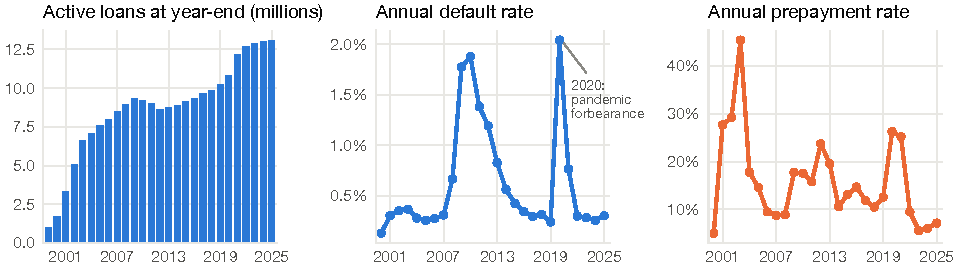
\includegraphics[width=\linewidth]{figures/data.pdf}
\caption{The Freddie Mac standard book. Left: loans active at each year-end.
Middle and right: share of active loans that default or prepay in the
following calendar year (default: first month 180+ days delinquent or a
credit-event zero balance).}
\label{fig:data}
\end{figure}

\subsection{Macro series}

House prices are the FHFA all-transactions index by state (FRED series
\texttt{\{ST\}STHPI}, quarterly), unemployment the BLS rate by state
(\texttt{\{ST\}UR}, monthly, seasonally adjusted), both for the 50 states and
the District of Columbia, and the market mortgage rate is Freddie Mac's PMMS
30-year fixed rate (\texttt{MORTGAGE30US}). A loan's origination month is
taken as two months before its first payment, because mortgage interest is
paid in arrears. The input at December $y$ uses the fourth-quarter index and
the December unemployment rate. Both are published in the first quarter of
$y+1$, before a December allowance is finalised. The checksums of the
downloaded series are in the repository.

\subsection{Judicial foreclosure}

Judicial-foreclosure states (Connecticut, Delaware, Florida, Iowa, Illinois,
Indiana, Kansas, Kentucky, Louisiana, Maine, North Dakota, New Jersey, New York,
Ohio, Pennsylvania, South Carolina, Vermont and Wisconsin) are those listed in
Table~2 of \citet{gerardi2013borrower}, whose assignment follows
\citet{rao2009foreclosing}. Foreclosure takes longer in these states. In the
severity tables (\cref{app:lgd}), judicial-state severity is the higher in
\num{data.jud.higher} of the \num{data.jud.n} band-and-date comparisons where
both cells have thirty or more resolutions; the exceptions are bands of 80\%
current LTV and above in 2008 to 2011.

\section{Method}\label{sec:method}

The design below was committed to the repository on 29 October 2026, before
any loan-level file had been downloaded (commit \texttt{07c8ffd}). The data log,
the deviations from it, the corrected bugs and the analyses added after the
results are listed in \cref{app:deviations}. Each choice is
stated with the reason for it.

\subsection{Reporting dates, portfolio and training data}

A reporting date $T$ is a calendar year-end, December 2005 to December 2025
(\num{const.n_dates} dates). The \emph{portfolio} at $T$ is every loan active
at December $T$: balance above zero, no zero-balance event, and never yet 180
or more days delinquent. Loans 30 to 179 days past due at $T$ are in the
portfolio, but current delinquency is not a model input (the design has
none), so the models treat them like current loans with the same inputs;
\cref{sec:limits} reports how much of the book they are. Allowances are computed on the \num{const.n_port}
portfolio loans with the smallest value of a fixed loan-level random draw,
and expressed as a rate, expected loss over balance on that sample (a ratio
estimator). The dollar figures multiply the rate by the balance of the whole
active book. \Cref{sec:sampling} reports the sampling error this adds.

A model at $T$ may use only what a lender knew at $T$, in the data as
published in 2026: Freddie Mac's Release 47 and current FRED vintages, which
may revise what was reported at the time (\cref{sec:limits}). Its training data are
the \emph{loan-years} whose outcome year ends on or before $T$: a loan active
at December $y \le T-1$ contributes one row, with inputs measured at December
$y$ and the outcome observed in year $y+1$. Censored loan-years (removal for a
defect or a reperforming sale, without a default first) are dropped. Loans,
never rows, are split by a keyed hash of the loan identifier: 20\% are held
out and used only to measure accuracy, 10\% are used for early stopping and
70\% for fitting. Each loan is kept with probability
$\min\{1, 6.25\text{M}/n_T\}$, where $n_T$ is the number of loan-years
available, so that fitting and early-stopping rows together are capped near
the design's five million.

\subsection{Outcomes, competing risks and inputs}

In each loan-year a loan defaults, prepays or survives. \emph{Default} is the
first month 180 or more days delinquent, or a credit-event zero balance
(third-party sale, short sale or charge-off, REO disposition, whole-loan
sale; codes 02, 03, 09, 15), whichever comes first. \emph{Prepayment} is a
voluntary payoff (code 01). Two binary hazard models describe the year:
\begin{equation}
h_d = \Pr(\text{default}\mid\text{active}),\qquad
h_p = \Pr(\text{prepay}\mid\text{active, no default}),
\end{equation}
so that $\Pr(\text{default})=h_d$, $\Pr(\text{prepay})=(1-h_d)h_p$ and
$\Pr(\text{survive})=(1-h_d)(1-h_p)$. Any three-outcome distribution factors
this way, and the multinomial log loss is exactly the sum of the two binary log
losses, so nothing is lost relative to a multinomial model. A single
multiclass gradient-boosting model was rejected because LightGBM applies a
monotone constraint in the same direction to every class's score, which would
force prepayment to rise with leverage as default does.

The \num{const.n_features} inputs are those in \cref{tab:features}: credit
score, original LTV and combined LTV, debt-to-income ratio, original rate and
its spread over the Freddie Mac PMMS 30-year rate in the origination month,
loan purpose, occupancy, property type, units, first-time-buyer flag, number
of borrowers, origination channel, mortgage-insurance percentage, original
term, loan age, \emph{current} LTV (current balance over the origination value
marked to the FHFA state house-price index), the state's house-price growth
over the prior year, and its unemployment rate and twelve-month change. Seller
and servicer names, ZIP3 and MSA are not used: they identify institutions or
come close to identifying places.

\subsection{The allowance}

For each portfolio loan the projection runs one row per remaining contractual
year $k=1,\dots,K$. The balance at the start of year $k$, $B_k$, is the
interest-bearing balance amortised at the loan's current rate over its
remaining term, plus any non-interest-bearing (deferred) balance, which is due
at maturity. Loan age advances by twelve months a year, current LTV follows
$B_k$ and the house-price path, and the origination inputs do not change.
With $S_1=1$,
\begin{equation}\label{eq:el}
m_k = S_k\,h_{d,k},\qquad S_{k+1}=S_k\,(1-h_{d,k})(1-h_{p,k}),\qquad
\mathrm{EL} = \sum_{k=1}^{K} B_k\, m_k\, \mathrm{LGD}_k ,
\end{equation}
where a final part-year of $q$ months uses $1-(1-h)^{q/12}$. The allowance is
undiscounted, the probability-of-default/loss-given-default method, which ASC
326 permits without discounting outside a discounted-cash-flow approach. The
lifetime PD of a loan is $\sum_k m_k$.

\paragraph{Macro path.} During the two-year reasonable and supportable period
the state's house-price growth and unemployment rate stay at their December $T$
values. Afterwards they revert to their long-run state means, computed over
all years up to $T$, in a straight line over one year (primary). The two
other policies of H2 are immediate reversion and straight-line reversion over
three years; ASC 326-20-30-9 names immediate and straight-line reversion, and
the durations are this study's choice. A loan-year beginning at year-end $p$
reads the path's value at $p$, as in training. Because the path is annual, the
first reverted value is at $T+3$ under both immediate and one-year
straight-line reversion, so those two policies give the same allowance and the
policy range of H2 is in effect the range between one- and three-year
reversion. The length of the reasonable and supportable period, also the
lender's choice, is held at two years throughout. A secondary
analysis replaces the forecast with the realized path through 2025.

\paragraph{Loss given default.} One severity model per date, held fixed across
all default models: total actual loss over total balance at default (a
balance-weighted severity), among defaults resolved by December $T$, by current-LTV band at the start of the
default year ($<$60, 60--80, 80--90, 90--100, 100--120, $\ge$120) and by
judicial-foreclosure state \citep{gerardi2013borrower}. A default
later paid off voluntarily has a loss of zero. A cell with fewer than thirty
resolutions uses its band's mean; a band with fewer than thirty uses the mean
of all resolutions. Actual loss is Freddie Mac's own calculation
\citep{FreddieGuide2026}.

\subsection{Models}

The default model is one of \num{const.n_models}, all trained on the same rows:
\begin{itemize}[nosep]
\item 32 LightGBM binary models \citep{ke2017lightgbm}: 15 or 63 leaves $\times$ four
row/column subsampling settings (80/100\% $\times$ 80/100\%), with five seeds
for each subsampled setting and one for the deterministic one;
\item the same 32 with monotone constraints: the default hazard may not fall as
current LTV or the debt-to-income ratio rises, or as the credit score falls;
\item one logistic regression on cubic splines of the numeric inputs (five
quantile knots) with one-hot categories.
\end{itemize}
LightGBM uses a learning rate of 0.1, at least 100 rows per leaf and early
stopping after 50 rounds without improvement on the early-stopping loans. The
prepayment model is fixed at each date: the most accurate on held-out
prepayment log loss among the eight unconstrained LightGBM settings (seed 1)
and the spline logit (Deviation~1).

\subsection{The set of equally accurate models}\label{sec:set}

Accuracy is held-out log loss of the default model, a proper scoring rule that
rewards calibration, which an allowance needs. Its sampling error is a
loan-clustered bootstrap: \num{const.n_boot} resamples of the held-out loans
with replacement. A model is in the set if its held-out log loss is within one
bootstrap standard error of the best. This is a tolerance,
not a test that the models are equal: a paired comparison on the same held-out
loans separates many of them from the best, and \cref{sec:sensitivity}
reports the much smaller sets such a test admits. The tolerance asks instead
which models a lender could not reject on accuracy measured as the lender
would usually measure it, one model at a time. Sensitivity analyses use half and two standard errors, and a set defined by
held-out AUC instead.

\subsection{Predictions}\label{sec:predictions}

Six predictions were recorded with the design, each with the result that
would refute it. They are reproduced here as written.

\begin{enumerate}[label=\textbf{H\arabic*.}, leftmargin=*, itemsep=2pt]
\item \emph{Model choice exceeds training noise.} At a majority of dates, the
range (max $-$ min) of the allowance across the set exceeds the 95\% interval
width of the best configuration's allowance across 20 refits on loan-level
bootstrap resamples of its training data.
\item \emph{Model choice rivals permitted policy discretion.} At a majority of
dates, the allowance range across the set is at least the range across the
three reversion policies ASC 326-20-30-9 names (immediate, straight-line over
one year, straight-line over three years), holding the best model fixed.
\item \emph{The spread widens into stress.} The allowance range as a share of
the best model's allowance is larger at year-ends 2006 and 2007 than at the
median of all other dates.
\item \emph{Constraints narrow the spread.} Within each family's own set (same
tolerance, relative to that family's best), the relative range is smaller for
monotone-constrained models than for unconstrained ones at a majority of dates.
\item \emph{The range is not forecast uncertainty.} For dates whose portfolio
has at least eight years of realized outcomes, realized lifetime credit losses
lie inside the range of allowances across the set at fewer than half of those
dates.
\item \emph{Staging flips.} Under the IFRS 9 analogue (lifetime PD at $T$ more
than twice the lifetime PD at origination as the significant-increase test),
the share of portfolio loans whose stage differs between at least two models
in the set exceeds the share whose stage differs across the 20 bootstrap
refits of H1, at a majority of dates.
\end{enumerate}

\noindent For H6 the lifetime PD at origination is computed by the same model
from the loan's origination inputs (age zero, original balance, rate and term,
current LTV equal to original LTV) and the macro values at the year-end before
its first payment, held for two years and then reverted as in the primary
path. A loan whose stage is the same under every model counts as stable. This
is a simplified analogue of the IFRS 9 test: it compares lifetime PDs from one
model, not the lender's own origination estimate; it compares the PD over the
remaining life with the PD over the full term, without the adjustment for the
shorter remaining life that IFRS 9 asks for (B5.5.11), which biases seasoned
loans towards stage 1; its origination path reverts to long-run means
computed at $T$; and it has no 30-days-past-due backstop.

\section{Results}\label{sec:results}

\subsection{Accuracy and the set of equally accurate models}

The most accurate default model is an unconstrained LightGBM model at every
date, with held-out AUC between \num{res.auc.min} and \num{res.auc.max}.
Accuracy differences across the grid are small next to the sampling error of
any one model's held-out log loss. The set therefore holds a median of
\num{res.set.size.median} of the \num{const.n_models} models (between
\num{res.set.size.min} and \num{res.set.size.max}), about \num{res.mono.share}\%
of them monotone-constrained. The spline logit is in the set only at the five
earliest dates. \Cref{fig:cloud} plots, at six dates, every model's held-out
log loss above the best (in standard errors) against its allowance relative
to the best. Within the shaded band of equal accuracy, allowances spread
widely.

\begin{figure}[t]
\centering
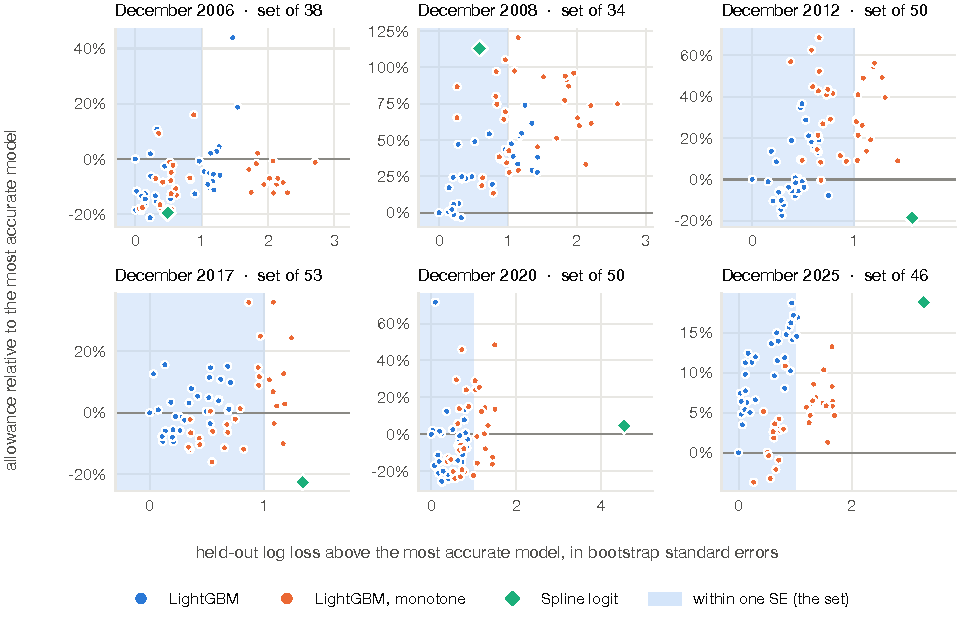
\includegraphics[width=\linewidth]{figures/cloud.pdf}
\caption{Accuracy and allowance for all \num{const.n_models} default models at
six reporting dates. Horizontal: held-out log loss above the most accurate
model, in bootstrap standard errors of that model's log loss. Vertical:
lifetime allowance relative to the most accurate model's. The shaded band is
the set of equally accurate models.}
\label{fig:cloud}
\end{figure}

\subsection{How far the allowance moves}\label{sec:sampling}

\Cref{fig:allowance}A shows the allowance across time. The most accurate
model's lifetime allowance runs from \num{res.best_rate.min}\% of balance to
\num{res.best_rate.max}\% (December \num{res.best_rate.max_year}). The range
across the set, as a share of the most accurate model's allowance, has a
median of \num{res.rel.median}\% across dates, from \num{res.rel.min}\% (December
\num{res.rel.min_year}) to \num{res.rel.max}\% (December \num{res.rel.max_year}).
Scaled to Freddie Mac's whole non-defaulted active book in the standard dataset, the range is
\num{res.usd.median} billion dollars at the median date and
\num{res.usd.max} billion dollars at December \num{res.usd.max_year}
(\cref{fig:dollars}). Drawing the 200{,}000 scored loans is not the source:
the bootstrap standard error of the allowance from that sampling has a median
of \num{res.samp_se.median_bp} basis points of balance, against a median range of
\num{res.range_bp.median} basis points. \Cref{tab:bydate} in
\cref{app:bydate} gives every date.

\begin{figure}[t]
\centering
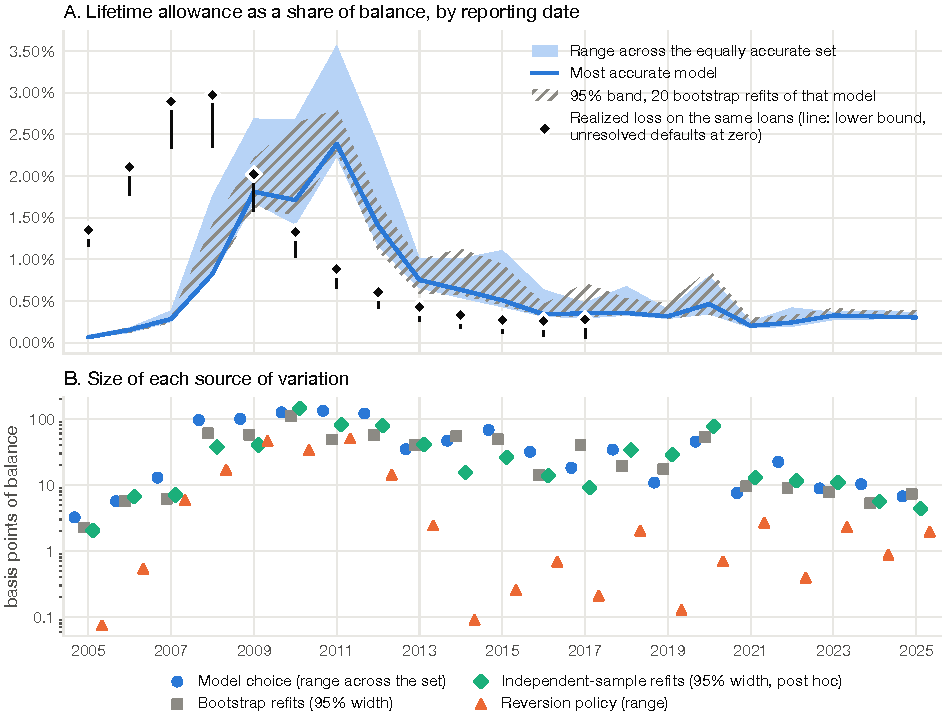
\includegraphics[width=\linewidth]{figures/allowance.pdf}
\caption{A: lifetime allowance as a share of the scored loans' balance, under
the primary forecast path and one-year straight-line reversion. The band is
the range across the set of equally accurate models; the hatched band the
central 95\% of 20 bootstrap refits of the most accurate configuration.
Diamonds: realized credit losses on the same loans for dates with at least
eight years of outcomes; the line below each diamond runs to the lower bound
in which defaults still unresolved in June 2026 carry no loss. B: the sources
of variation in basis points of balance (log scale); the independent-sample
refits of \cref{sec:refits} were added after the results.}
\label{fig:allowance}
\end{figure}

\begin{figure}[t]
\centering
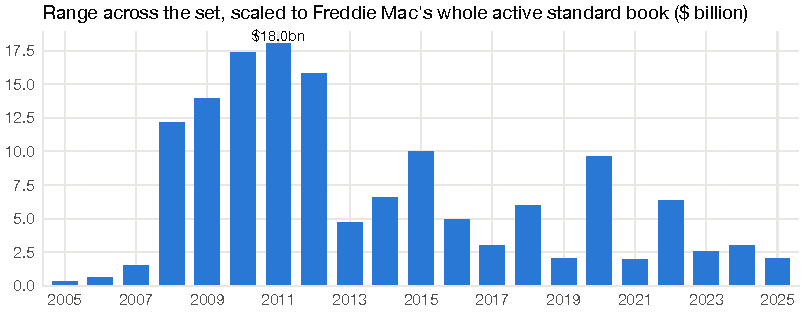
\includegraphics[width=\linewidth]{figures/dollars.pdf}
\caption{Range of the allowance across the set of equally accurate models,
multiplied by the balance of every loan active in Freddie Mac's standard
dataset at each year-end.}
\label{fig:dollars}
\end{figure}

\subsection{The six predictions}

\begin{table}[t]\centering\small
\caption{The six predictions recorded before the data were opened, as tested.}\label{tab:hyp}
\begin{tabular}{llll}\toprule
& Prediction & Evidence & Verdict \\ \midrule
H1 & Model choice $>$ refit noise & 13 of 21 dates & Holds \\
H2 & Model choice $\ge$ reversion range (1 vs 3 years) & 21 of 21 dates & Holds \\
H3 & Relative range larger at 2006 and 2007 & 37\%, 46\% vs 56\% & \textbf{Fails} \\
H4 & Monotone family narrower & 12 of 21 dates & Holds \\
H5 & Realized loss inside the range at $<$ half & 1 of 13 dates & Holds \\
H6 & Stage flips $>$ refit flips & 17 of 21 dates & Holds \\
\bottomrule\end{tabular}
\end{table}


\Cref{tab:hyp} summarises the verdicts. Two of them, H1 and H6, depend on
how the tests were built, and \cref{sec:likeforlike} reports like-for-like
versions.

\paragraph{H1 (model choice exceeds refit noise) \num{H1.verdict}.} The
range across the set exceeds the 95\% width of 20 bootstrap refits at
\num{H1.n} of \num{const.n_dates} dates, with a median ratio of
\num{res.ratio_refit.median}. Training noise is large in its own right: at
several dates refitting the best configuration on resampled loans moves the
allowance by more than half its level (\cref{fig:allowance}A). The bootstrap
refits the test uses are a weaker benchmark than the design intended,
however; \cref{sec:refits} shows that refits on independent samples, which do
not share that weakness, span at least as much as the set.

\paragraph{H2 (model choice rivals the reversion policy) \num{H2.verdict}.} At
\num{H2.n} of \num{const.n_dates} dates the range across the set is at least
the range across the three reversion policies, with a median ratio of
\num{res.ratio_policy.median}. Immediate and one-year straight-line reversion
give the same annual path (\cref{sec:method}), so this is the range between
one- and three-year reversion, and the discretion over the length of the
forecast period, which is not varied here, would add to it. The policy matters
most when the economy at $T$ is far from its long-run average: its range is a
median of \num{res.policy.rel.median1}\% of the allowance, but
\num{res.policy.rel.gfc.min}\% to \num{res.policy.rel.gfc.max}\% at the
year-ends 2008 to 2011, \num{res.policy.rel.2007}\% at December 2007 and
\num{res.policy.rel.2021}\% at December 2021. The choice among
equally accurate models matters at every date (\cref{fig:allowance}B).

\paragraph{H3 (the spread widens into stress) \num{H3.verdict}.} The relative
range is \num{H3.rel2006}\% at December 2006 and \num{H3.rel2007}\% at December
2007, below the \num{H3.median}\% median of the other dates (\cref{fig:relative}).
On the eve of the crisis the models' disagreement was ordinary in relative
terms. It is the level of the allowance that was badly wrong, and the
absolute range then grew with it: in dollars the spread was largest from 2008
to 2012 (\cref{fig:dollars}).

\begin{figure}[t]
\centering
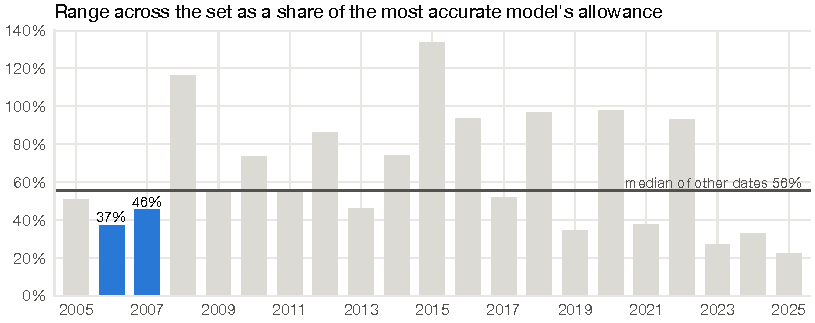
\includegraphics[width=\linewidth]{figures/relative.pdf}
\caption{Range across the set as a share of the most accurate model's
allowance. H3 predicted the two highlighted dates would exceed the median of
the others.}
\label{fig:relative}
\end{figure}

\paragraph{H4 (constraints narrow the spread) \num{H4.verdict}, narrowly.}
Within each family's own set, the monotone-constrained models have the
smaller relative range at \num{H4.n} of \num{const.n_dates} dates
(\cref{fig:families}A), one more than a majority. They do not narrow it on
average: the median relative range is \num{res.fam.mono.median}\% for the
constrained family and \num{res.fam.lgbm.median}\% for the unconstrained one.
Constraints that encode the
expected direction of credit risk do not reliably tie down the lifetime
allowance; most of the lifetime projection runs through inputs they leave free
(loan age, the macro path, the interaction of default with prepayment).
The two families' sets differ in size, and a range grows with the number of
models in it; comparing random subsets of equal size (added after the
results) leaves the verdict unchanged, with the constrained family narrower at
\num{p2.h4.n} dates and medians of \num{p2.h4.mono}\% and \num{p2.h4.lgbm}\%.

\paragraph{H5 (the range is not forecast uncertainty) \num{H5.verdict}.} For the
\num{H5.n_elig} reporting dates with at least eight years of outcomes
(\num{H5.first} to \num{H5.last}), realized credit losses on the scored loans lie
inside the set's range at \num{H5.inside} date (December 2009), and at none when
unresolved defaults are counted at zero. They lie above the range at the
\num{H5.above} dates from 2005 to 2008 and below it at the \num{H5.below} dates
from 2010 to 2017. Two caveats qualify the comparison. Outcomes are observed
only to June 2026, so the realized loss of the later portfolios is truncated
while the allowance is lifetime; the horizon-matched comparison (losses and
allowances both through 2025) puts realized losses inside the range at
\num{H5.inside25} dates. And a growing share of the later realized losses is
imputed for defaults not yet resolved (\cref{tab:decomp}, last column).

The range across equally accurate models says nothing about forecast error:
realized losses on the December 2006 portfolio were \num{res.miss2006} times
the top of the set's range, while the models agreed with one another far more
closely than with the outcome. \Cref{tab:decomp}, added after the results,
splits the miss for the most accurate model. Before the crisis the forecast
held each state's house-price growth at its December value (a median
\num{mac.hpi2005}\% a year at December 2005 and \num{mac.hpi2006}\% at December
2006) and the severity table reflected a benign history. Replacing the
forecast with the realized macro path raises the 2005--2008 allowances by a
factor of \num{dec.path.min} to \num{dec.path.max}. Replacing the severity
table with that of the defaults resolved by December 2019, after the crisis
losses and before pandemic forbearance, raises them by a further
\num{dec.lgd19.min} to \num{dec.lgd19.max} times (column 3). The result is
within \num{dec.lgd19.short.max}\% of realized losses at 2005, 2007 and 2008
and \num{dec.lgd19.over2006}\% above them at 2006. The default model itself was
not the main problem: on the realized path its mean lifetime PD is
\num{pd.pre.min} to \num{pd.pre.max} times the share of loans that actually
defaulted at the four pre-crisis dates. The miss came from the forecast and
from severities estimated on a benign history. The severity table of December
2025 (column 4) is a poorer guide to crisis losses, because it counts the
payoffs after pandemic-era ``defaults'' as zero-loss resolutions.

After the crisis the order reverses. The forecast held the high unemployment
of the years after 2009, and from December 2011 the realized path and the
2019 severities each lower the allowance, but column (3) still exceeds
realized losses at every date from 2010 to 2017. The defaults are not the
reason: for the 2013 to 2017 portfolios the model's lifetime PD is only
\num{pd.late.min} to \num{pd.late.max} times the realized default share, which
the pandemic forbearance ``defaults'' inflate. Those defaults resolved with
little loss, which no severity table estimated before 2020 anticipates;
column (4) is closer to realized losses from 2010 to 2015, partly mechanically, since the
imputed part of realized loss is valued at much the same diluted severities.
With the realized macro path
in place of the forecast, the set's range widens to a median of
\num{res.realpath.rel.median}\% of the best model's allowance, so the models
disagree most when the economy moves outside the training data.

\begin{table}[t]\centering\footnotesize
\caption{Where the miss comes from (added after the results). Lifetime allowance of the most accurate model, \% of balance: (1) primary forecast and the severity table at $T$; (2) realized macro path, severity at $T$; (3) realized path and the severity table of defaults resolved by December 2019, before pandemic forbearance; (4) realized path and the table of defaults resolved by December 2025, which counts pandemic-era payoffs after default as zero-loss resolutions. Realized loss: recorded estimate, lower bound with unresolved defaults at zero, and the imputed share, valued at the severity of all resolutions through June 2026. Defaults: the model's mean lifetime PD on the realized path, and the share of loans that defaulted by June 2026.}\label{tab:decomp}
\setlength{\tabcolsep}{3.5pt}
\begin{tabular}{rrrrrrrrrr}\toprule
& \multicolumn{4}{c}{Allowance} & \multicolumn{3}{c}{Realized loss} & \multicolumn{2}{c}{Defaults (\%)} \\
\cmidrule(lr){2-5}\cmidrule(lr){6-8}\cmidrule(lr){9-10}
Dec. & (1) & (2) & (3) & (4) & Est. & Lower & Imp.\,\% & PD & Actual \\ \midrule
2005 & 0.06 & 0.32 & 1.19 & 0.92 & 1.35 & 1.15 & 14 & 3.8 & 5.1 \\
2006 & 0.15 & 0.76 & 2.48 & 1.85 & 2.11 & 1.77 & 16 & 8.6 & 6.3 \\
2007 & 0.28 & 0.74 & 2.24 & 1.75 & 2.90 & 2.34 & 19 & 6.6 & 7.6 \\
2008 & 0.83 & 1.06 & 2.42 & 1.91 & 2.98 & 2.34 & 22 & 7.4 & 7.8 \\
2009 & 1.81 & 1.59 & 2.19 & 1.78 & 2.02 & 1.57 & 22 & 6.4 & 6.3 \\
2010 & 1.71 & 1.74 & 1.91 & 1.57 & 1.33 & 1.02 & 23 & 5.6 & 4.9 \\
2011 & 2.39 & 1.50 & 1.47 & 1.19 & 0.88 & 0.65 & 27 & 4.5 & 3.9 \\
2012 & 1.41 & 1.12 & 1.06 & 0.84 & 0.61 & 0.41 & 32 & 3.5 & 3.4 \\
2013 & 0.75 & 0.63 & 0.60 & 0.45 & 0.43 & 0.26 & 40 & 2.4 & 3.0 \\
2014 & 0.63 & 0.52 & 0.49 & 0.35 & 0.33 & 0.17 & 50 & 2.2 & 2.7 \\
2015 & 0.51 & 0.44 & 0.41 & 0.28 & 0.27 & 0.10 & 62 & 2.0 & 2.6 \\
2016 & 0.34 & 0.31 & 0.29 & 0.20 & 0.26 & 0.07 & 75 & 1.5 & 2.8 \\
2017 & 0.35 & 0.33 & 0.32 & 0.20 & 0.28 & 0.04 & 85 & 1.9 & 2.9 \\
\bottomrule\end{tabular}
\end{table}


\paragraph{H6 (staging flips) \num{H6.verdict}.} At \num{H6.n} of
\num{const.n_dates} dates more loans change IFRS 9 stage across the set than
across the refits, but the medians are almost equal: \num{res.flip.median}\% of
loans across the set and \num{res.flip_refit.median}\% across the refits
(\cref{fig:families}B). The prediction holds as recorded, but the
like-for-like comparisons of \cref{sec:refits} contradict the reasoning
behind it: refits change at least as many loans' stage as model choice. The share of loans in stage 2 under the best model
runs from \num{res.stage2.min}\% to \num{res.stage2.max}\%. Many loans sit near
the twice-the-origination-PD threshold, so any model change moves some of them
across it.

\begin{figure}[t]
\centering
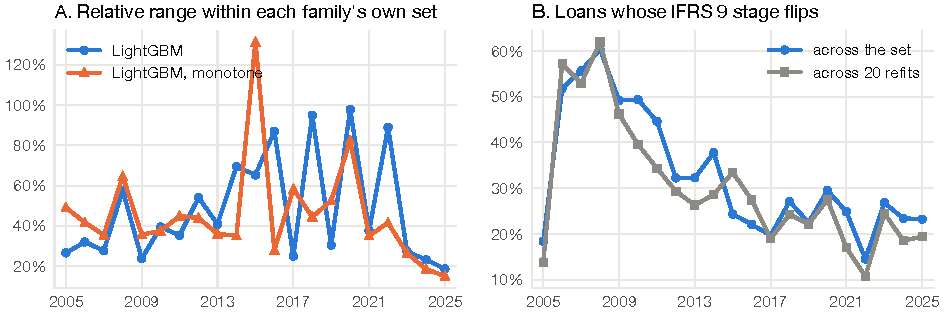
\includegraphics[width=\linewidth]{figures/families_stages.pdf}
\caption{A: H4, the relative range within each LightGBM family's own set of
equally accurate models. B: H6, the share of scored loans whose IFRS 9 stage
(lifetime PD more than twice its origination value) differs between at least
two models of the set, and between at least two of the 20 refits.}
\label{fig:families}
\end{figure}

\subsection{Refit noise, like for like (added after the results)}\label{sec:likeforlike}\label{sec:refits}

H1 and H6 as recorded have two weaknesses, both found after the results.
First, they compare a range or a disagreement among about fifty set models
with a central interval or a disagreement among twenty refits, so both lean
towards the set. Second, the recorded refits fit on bootstrap resamples of the
training loans, implemented as integer case weights; a resample contains
about 63\% of the distinct loans, and LightGBM's minimum leaf size and row
subsampling count rows, not weights. The refits are less accurate than the
model they refit: their held-out log loss is a median \num{ph.rq.gap} standard
errors above the best model's, \num{ph.rq.gt1} of the \num{ph.rq.total} refits
(\num{ph.rq.gt1.share}\%) would fall outside the set's tolerance, and their
mean allowance exceeds the best model's at \num{ph.rq.above} of
\num{const.n_dates} dates (median \num{ph.rq.bias}\%).

Two analyses address this. Twenty models are drawn at random from the set,
and the best configuration is refitted on twenty random samples of the panel,
each the same size as its original fitting sample, with the same fitting and
early-stopping split and the same held-out loans for accuracy. These refits
are as accurate as the original to within a fraction of a standard error
(median gap \num{ph.rs.gap}), so each is a model the lender could have fitted
and kept. The samples are windows of a uniform loan-level draw. When the
sampling fraction is below 1/21, at the \num{ph.rs.disj.n} dates from December
\num{ph.rs.disj.first}, they are disjoint from one another and from the
original. At earlier dates neighbouring windows overlap, by up to
\num{ph.rs.mut.max}\% of their loans (December \num{ph.rs.mut.max_year}), and
share at most \num{ph.rs.ov.max}\% with the original on average. Overlap
narrows the refits' spread, so the comparison is cleanest at the disjoint
dates.

There, training-sample noise exceeds model choice: twenty refits span a median
\num{p2.disj.rsm}\% of the allowance against \num{p2.disj.lfl}\% for twenty set
models, and more at \num{ph.rs.disj.refitmore} of the \num{ph.rs.disj.n}
dates. Over all dates, including those where overlap holds the refits back,
the two are equal: medians of \num{ph.rs.rel.median}\% and \num{ph.lfl.rel.median}\%, with
the set's twenty wider at \num{ph.rs.n} of \num{const.n_dates} dates (median
ratio \num{ph.rs.ratio}). Rerun against these refits, the recorded H1 test
(the set's full range against the refits' central 95\% width) would hold at
\num{ph.rs.w95} dates. Bootstrap refits span a median \num{p2.boot.rel}\%, more
than the independent refits at only \num{p2.boot_gt_rsm} dates, so their flaw
is inaccuracy and bias rather than a wider spread. For staging the comparison
is one-sided: the independent-sample refits flip a median \num{ph.rs.flip}\%
of loans' IFRS 9 stage against \num{ph.H6.flipset}\% for twenty set models, and
fewer at only \num{ph.rs.flipmore} dates.

The training samples here are capped near five million loan-years, which is
\num{ph.frac.min}\% of the history available at December
\num{ph.frac.min_year}. Fitting on all of Freddie Mac's history would shrink
this noise. A bank fitting on its own, much smaller, book would face more.

\paragraph{Where the most accurate model sits.} The most accurate model is in
the lower part of the set's range: a median \num{p2.pos.median}\% of the way
from the lowest allowance to the highest, below the set's median at
\num{p2.below_median} of \num{const.n_dates} dates, though the set's median is
only a median \num{p2.median_gap}\% above it. The range is skewed upward, with a
few models giving much higher allowances. Across the set, held-out log loss
and allowance are positively rank-correlated at \num{p2.rho_set.pos} dates
(median Spearman correlation \num{p2.rho_set.median}): the more accurate
models give lower allowances. Across the twenty refits of one configuration
the correlation is a median \num{p2.rho_rsm.median}, so picking the lowest
log loss does not select a low allowance by chance within a configuration.
The refits' mean allowance nonetheless exceeds the best model's at
\num{ph.rs.bias.pos} of \num{const.n_dates} dates (median \num{ph.rs.bias}\%).
The original sample is the same loan-level draw at every date, so these
dates are not independent observations of that gap, and it is left
unexplained. For SAB 119 the point is practical: a booked estimate from the
most accurate model sits in the lower part of the identified range.

The honest reading is that the allowance is at least as sensitive to which
loans happen to be in the training sample as to which of several equally
accurate configurations is chosen, and IFRS 9 staging more so. Both are model
uncertainty of the kind SAB 119's ``identified range'' asks a registrant to
document, and neither appears in a single best estimate.

\subsection{Sensitivity}\label{sec:sensitivity}

\paragraph{The tolerance.} \Cref{fig:sensitivity} recomputes the relative
range with the tolerance at half and two standard errors and with a set
defined by AUC: medians of \num{res.rel05.median}\%, \num{res.rel2.median}\% and
\num{res.relauc.median}\% against \num{res.rel.median}\% for the recorded set.
A much stricter set, added after the first results, admits a model only if
its held-out log loss is within two bootstrap standard errors of its
\emph{paired} difference from the best; it holds a median of
\num{ph.paired2.size} models, and its relative range still has a median of
\num{ph.paired2.rel}\%. With one paired standard error the set has a median of
\num{res.paired1.size} models and a median relative range of
\num{res.paired1.rel}\%.

\paragraph{The prepayment model.} Letting the prepayment model vary over its
own set as well (every pair of default and prepayment models) gives a median
relative range of \num{res.both.rel.median}\%, against \num{res.rel.median}\%
with the prepayment model fixed. The default model carries the spread.

\begin{figure}[t]
\centering
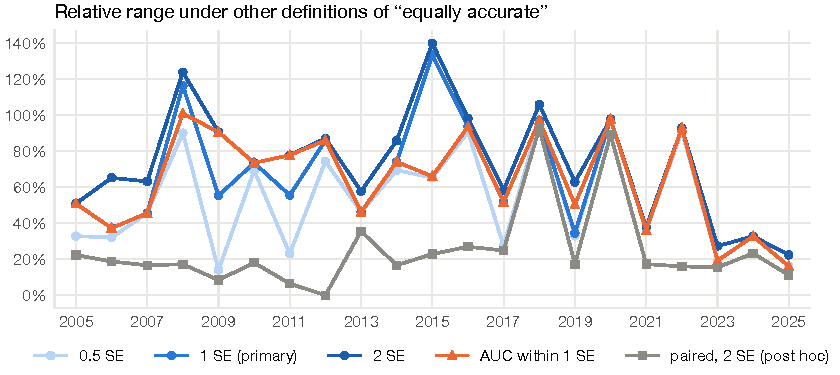
\includegraphics[width=\linewidth]{figures/sensitivity.pdf}
\caption{Relative range of the allowance across the set under other
definitions of equal accuracy. ``Paired'' admits models within two bootstrap
standard errors of their paired difference in held-out log loss from the best
(added after the results).}
\label{fig:sensitivity}
\end{figure}

\subsection{Where loans disagree}

The loan-level spread is large even where the aggregate range is modest. For
each scored loan, \cref{fig:loans} takes the ratio of its largest to smallest
lifetime PD across the set. Taking the median loan's ratio at each date
and then the median across dates, it is between \num{res.loan.ratio.min} and
\num{res.loan.ratio.max} in every LTV and credit-score band, and it is largest for the safest loans (current LTV below
60\% and credit scores of 760 or more), whose PDs are smallest. In
percentage points the spread is largest for loans in negative equity.
Disagreement in a sum over two hundred thousand loans partly cancels, which
is why the portfolio range is narrower than the loan-level ranges.

\begin{figure}[t]
\centering
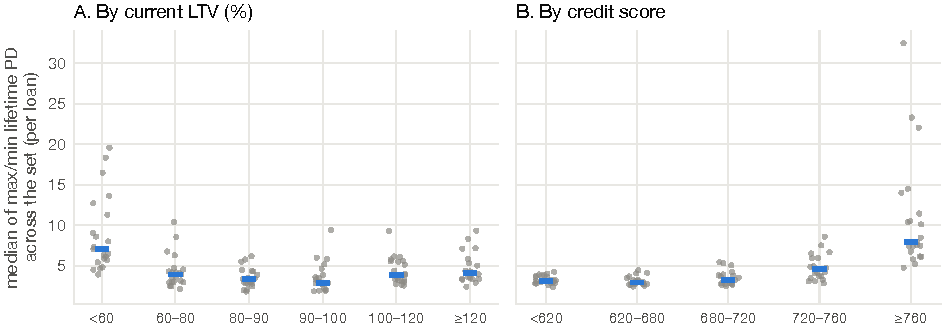
\includegraphics[width=\linewidth]{figures/loans.pdf}
\caption{Per loan, the ratio of the largest to the smallest lifetime PD
across the set; grey dots are the medians at each reporting date, the bar
the median across dates.}
\label{fig:loans}
\end{figure}

\section{Discussion}\label{sec:discussion}

\subsection{What the range means for preparers, auditors and validators}

\paragraph{Preparers.} SAB 119 expects a registrant to document an identified
range of expected credit losses and its reasons for the point it books. The
results suggest the range should include the model. On this book a median
of \num{res.rel.median}\% of the allowance separates models within one standard
error of the best held-out log loss (\num{ph.paired2.rel}\% under a strict
paired test), and retraining the chosen model on another random sample of the
same size moves it at least as far. A lender can measure both with the procedure
here: fit a small grid, keep the models within a stated tolerance of the best
held-out log loss, refit the best on independent samples of its data, and
report the allowance across both. Bootstrap refits are a poor substitute:
they are less accurate than the model they refit and biased upward. None of this needs data the lender does not already have.

\paragraph{Auditors.} AS 2501 asks the auditor to evaluate the company's
selection among reasonable alternatives, and AS 2810 treats a recorded
estimate outside a reasonable range as misstated by the distance to the closest
reasonable estimate. Equally accurate models are reasonable alternatives on
any accuracy-based standard. A set like the one used here gives the auditor a
reproducible range to set the booked estimate against, in place of a judgment
about whether a single model is ``reasonable''.

\paragraph{Model validators.} The 2026 interagency guidance asks validators to
benchmark against alternative models, but it does not address accounting
estimates. Benchmarking that compares a chosen model with alternatives only on
accuracy will pass every model in the set while missing the
\num{res.rel.median}\% spread in what the models are for. Validation of an
allowance model should compare allowances, not only accuracy, across the
models the bank could defensibly have chosen, and include refit noise.

\paragraph{Monotone constraints are not a fix.} Constraining the direction of
credit risk narrowed the range at barely more than half the dates (H4), and
not at all on average. The lifetime projection runs through inputs the
constraints leave free.

\paragraph{No range is forecast uncertainty.} At all but one of the
dates with eight or more years of outcomes, the realized loss on the scored
loans lay outside the set's range (H5), and outside the range of the refits at
all but \num{p2.in_refit} (bootstrap) or \num{p2.in_rsm} (independent samples). Before the crisis every model in the
set, fed a forecast that held house prices rising at their 2005 or 2006 pace
and a severity table from benign years, missed the losses by a wide margin;
after it the allowance overshot. Before the crisis the miss lay in the
forecast and the severity table rather than in the default model, whose
lifetime PDs on the realized path were close to the realized default rates
(\cref{tab:decomp}), and the models agreed with one another far more than
with the outcome. A range across models documents one kind of uncertainty
and should not be read as a confidence interval for losses.

\subsection{Limitations}\label{sec:limits}

\begin{itemize}[leftmargin=*, itemsep=2pt]
\item \emph{One book, one product.} The data are Freddie Mac's standard dataset
of conforming, fully amortizing fixed-rate mortgages. Banks' books contain
other products, and an agency guarantor bears credit risk differently from a
bank holding a loan. The magnitudes should not be read as a bank's; the
procedure carries over.
\item \emph{No delinquency input.} The design has no current-delinquency
input. Loans 30 to 179 days past due are \num{dq.share.min}\% to
\num{dq.share.max}\% of the portfolio balance (most in December
\num{dq.share.max_year}), and they default far more often than current loans:
in 2010, \num{dq.2009.d90}\% of the loans 90 to 179 days past due at December
2009 defaulted and \num{dq.2009.d30}\% of those 30 to 89 days past due, against
\num{dq.2009.cur}\% of current loans. Any lender would use delinquency, which
would raise the level of the allowance, most in 2008 to 2011. Whether it
would narrow the range across models is not tested here.
\item \emph{The tolerance.} The recorded set admits models within one
bootstrap standard error of the best model's own log loss, which is generous:
a test on paired differences admits a median of \num{ph.paired2.size} models at
two standard errors. The relative range is still \num{ph.paired2.rel}\% of the
allowance under that strict set.
\item \emph{The model grid.} The set contains only the families tried here.
A wider grid (neural networks, other link functions) could widen the range,
which is therefore a lower bound on model-choice uncertainty within these
families.
\item \emph{The policy range.} At annual resolution two of the three reversion
policies coincide, and the length of the forecast period is not varied, so
H2 compares the model range with a narrow slice of the policy discretion the
standard allows.
\item \emph{Data as revised.} Each date uses only data dated on or before $T$,
but in its 2026 form: (a) Freddie Mac's Release 47 performance history and actual losses,
which may correct what was reported at the time and include recoveries and
expenses posted after a loan's zero-balance date, so the severity table at $T$
contains amounts a lender at $T$ had not yet seen; (b) current FRED vintages
of the house-price index and unemployment rates, which are revised; (c)
long-run means that include year $T$ itself; (d) the exclusion from the
severity table of loans repurchased for a defect found after $T$. None of
these is a default outcome after $T$, but (a), (b) and (d) are information a
lender at $T$ did not have in this form.
\item \emph{Censored loan-years.} Loan-years ending in removal for a defect or
a reperforming sale without a prior default are dropped from training, which
treats that removal as uninformative about default.
\item \emph{Pandemic forbearance.} By the recorded definition, a loan 180 days
past due in forbearance has defaulted. Models trained after 2020 learn that
spike, and most of those loans were later paid off or remain active. This
raises lifetime PDs at the later dates; the severity table offsets it in part
because payoffs after default count as zero-loss resolutions.
\item \emph{Severity.} The loss-given-default table is held fixed across
models, uses only defaults resolved by the reporting date, and excludes
modification costs, which Freddie Mac's actual-loss field omits. The design's
secondary analysis that lets severity vary with the default model was not run
(\cref{app:deviations}); a model for severity would add another source of
variation.
\item \emph{Realized losses.} Outcomes end in June 2026, so the realized loss
of the later portfolios is truncated. Defaults still unresolved then are
valued at the severity of resolved defaults, which is most of realized loss
from 2015 (\cref{tab:decomp}); the lower bound counts them at zero. Neither
changes the verdict on H5.
\end{itemize}

\subsection{Conclusion}

The CECL standard leaves the method to the lender, and the evidence here is
that the choice is not innocuous. Equally accurate default models trained on
the same history give allowances a median \num{res.rel.median}\% apart, more
than the gap between one- and three-year reversion, and no more than
retraining one model on another sample of its loans. Neither source of
variation tells a lender where losses will land. Documenting the range from
the model, as SAB 119 already asks for the estimate, is cheap with the
procedure released here, and it is the part of the identified range a bank
can measure with its own data.

\section{Code and data availability}\label{sec:availability}

The repository,
\href{https://github.com/ayk5511/eclrange}{github.com/ayk5511/eclrange}, holds
the code (MIT licence) and the text, tables, figures and aggregate results
(CC BY 4.0). It contains:
\begin{itemize}[nosep]
\item the pipeline, \texttt{code/01\_ingest.py} to \texttt{code/09\_paper.py},
which rebuilds every derived file from the Freddie Mac year archives and FRED
series (the SHA-256 checksums of both are listed in \texttt{data/}), and
\texttt{code/09\_paper.py}, which writes every number and table the paper
prints;
\item the recorded design, its commit date and the deviations, in the
repository's \texttt{README.md};
\item every per-date aggregate the paper reads (accuracy of each model, its
allowance under each path and policy, severity tables, realized losses) and
\texttt{paper/audit.py}, which recomputes the paper's numbers from them with
independent code;
\item unit tests of the allowance arithmetic (\texttt{tests/}).
\end{itemize}
No loan-level record or loan-level derivative is released: the Freddie Mac
terms permit publishing research results only where they cannot be used to
recreate the data \citep{FreddieTerms2025}. Anyone who registers with Freddie
Mac can download the same archives and rerun the pipeline. On an 18-core
workstation with 128 GB of memory the ingest takes about 40 minutes and the
models and allowances about \num{const.hours} hours.


\bibliographystyle{apalike}
\bibliography{bib/references}

\appendix
\section{Inputs}\label{app:features}

\begin{table}[H]\centering\small
\caption{Model inputs, measured at December of the snapshot year.}\label{tab:features}
\begin{tabularx}{\linewidth}{>{\raggedright\arraybackslash}p{5.2cm}X}\toprule
Input & Definition \\ \midrule
Credit score & Borrower credit score at origination (missing if not disclosed) \\
Original LTV, CLTV & Loan-to-value and combined loan-to-value at origination (\%) \\
Debt-to-income & Back-end ratio at origination (\%; missing above 65) \\
Original rate; spread & Note rate; note rate minus the PMMS 30-year rate in the origination month \\
Purpose, occupancy, property type, channel, first-time buyer & Categorical, as disclosed \\
Units; number of borrowers & As disclosed \\
MI percentage & Mortgage-insurance coverage at origination \\
Original term & Months \\
Loan age & Months since the first payment date, plus one \\
Current LTV & Current balance over (original balance / original LTV) $\times$ state HPI now / state HPI at origination \\
HPI growth & State FHFA index, fourth quarter over fourth quarter \\
Unemployment; change & State rate in December; change over twelve months \\
\bottomrule
\end{tabularx}
\end{table}

\section{Data log, deviations, corrections and added analyses}\label{app:deviations}

The design was committed at 10:36 ET on 29 October 2026 (commit
\texttt{07c8ffd}); the year archives were downloaded between 13:25 and 14:30
ET the same day, and the first loan-level file was opened at 14:33 ET to read
the Release 47 layout. The commit timestamp is the author's machine time; it
is not a third-party registration.

\paragraph{Deviation 1: prepayment grid.} The design chose the prepayment
model as the best of the full 65-model grid. A timing probe at December 2008,
before any allowance had been computed, showed that a prepayment LightGBM
model runs to about 2,700 boosting rounds (about 100 seconds), so the full grid
would have cost about two hours per date. The prepayment model is instead the
best of the eight unconstrained LightGBM settings at seed 1 and the spline
logit. The design's monotone constraints are written for default risk and
would force prepayment to fall as the credit score rises; extra seeds only
choose the luckiest draw of a model the design holds fixed. The grid of
default models, which is what the study is about, is unchanged.

\paragraph{Implementation details the design did not specify.} Early stopping
uses a further 10\% of loans (so fitting uses 70\%). A final part-year hazard
is scaled as $1-(1-h)^{q/12}$. The LGD table falls back to the band, then the
overall, mean for cells with fewer than 30 resolutions. A default later
repaid voluntarily is a zero-loss resolution; defaults removed by a
reperforming sale or a defect, or with no disclosed loss, are not used in the
severity table. The IFRS 9 origination projection is defined in
\cref{sec:predictions}. All of these were fixed before any allowance was
computed.

\paragraph{Deviations 2 to 4.} (2) The design listed a secondary analysis in
which severity varies with the default model; it was not run, and severity is
held fixed throughout. (3) The design scales the scored sample's allowance by
the inverse sampling fraction; the code uses the ratio estimator (expected
loss over balance on the sample, times the balance of the whole active
book), which agrees in expectation and has lower variance. (4) The design
computes the reversion means ``on data before $t$''; the code uses every year
up to and including $T$, whose December values are observed at $T$.

\paragraph{Corrections.} Four bugs were found while checking results and
fixed; the affected steps were rerun for every date, and every number in the
paper comes from the corrected code. The fitted models were not affected by
any of them. (1) The realized macro path looked up each state with the wrong
key and fell back to the long-run means. (2) A few dozen loans a year with no
remaining term were cast to invalid integers; they now use the original term
less the months paid. Both were found after the first three dates'
allowances. (3) The severity table first averaged per-loan ratios of loss to
balance at default, which a handful of loans with near-zero balances at
default dominate (one with \$0.19 at default and a \$27{,}168 loss); severity
is now balance-weighted, total loss over total balance at default. This was
found after every date's allowance existed, from an implausible level.
(4) Found by an independent review: ``immediate'' reversion set the macro
value at year-end $T+2$ to the long-run mean, which, because that value is
the house-price growth over year $T+2$, shortened the two-year forecast
period. Immediate reversion now starts at $T+3$ (\cref{sec:method}).

\paragraph{Analyses added after seeing results.} Each is labelled in the text
and none replaces a recorded test: (1) the paired-difference tolerance
(\cref{sec:sensitivity}); (2) the like-for-like versions of H1 and H6 and
(3) the refits on independent samples, with the accuracy and bias of both
kinds of refit (\cref{sec:refits}); (4) the lower bound for realized losses,
which counts defaults unresolved in June 2026 at zero; (5) the decomposition
of the H5 miss (\cref{tab:decomp}); (6) the delinquency of the portfolio
(\cref{sec:limits}); (7) the position of the most accurate model in the set,
the rank correlation of accuracy with the allowance, H4 on equal-size sets,
the refit ranges against realized losses, and the decomposition with the
December 2019 severity table and the realized default rates
(\texttt{code/07b\_posthoc.py}). Items (3), (5) and (6), and bug (4),
followed an independent referee review of a complete draft, and item (7) a
second one.

\section{Severity tables}\label{app:lgd}

\begin{table}[H]\centering\footnotesize
\caption{Loss given default (\% of balance at default) by current-LTV band at the start of the default year; P = power of sale, J = judicial. $^\dagger$ fewer than 30 resolutions in the cell, so the band or overall mean is used.}\label{tab:lgd}
\setlength{\tabcolsep}{3.5pt}
\begin{tabular}{rrrrrrrrrrrrr}\toprule
Dec. & \multicolumn{2}{c}{$<$60} & \multicolumn{2}{c}{60--80} & \multicolumn{2}{c}{80--90} & \multicolumn{2}{c}{90--100} & \multicolumn{2}{c}{100--120} & \multicolumn{2}{c}{$\ge$120} \\
 & P & J & P & J & P & J & P & J & P & J & P & J \\ \midrule
2006 & 3 & 6 & 11 & 17 & 7 & 12 & 5 & 8 & 10$^\dagger$ & 10$^\dagger$ & 10$^\dagger$ & 10$^\dagger$ \\
2008 & 7 & 9 & 17 & 22 & 12 & 15 & 9 & 10 & 20 & 20 & 15$^\dagger$ & 15$^\dagger$ \\
2012 & 15 & 20 & 31 & 38 & 39 & 42 & 40 & 41 & 48 & 52 & 46 & 47 \\
2017 & 14 & 24 & 28 & 41 & 35 & 47 & 36 & 45 & 41 & 52 & 42 & 48 \\
2025 & 7 & 14 & 18 & 28 & 26 & 37 & 30 & 39 & 39 & 49 & 40 & 47 \\
\bottomrule\end{tabular}
\end{table}


\section{Results by reporting date}\label{app:bydate}

\begin{table}[H]\centering\footnotesize
\caption{Allowance by reporting date. Rates are lifetime expected loss as a percentage of balance on the scored sample; set range in \% of balance; refit and policy widths in basis points of balance; \$ range scales the set's range to the whole active book. Realized loss in parentheses where fewer than eight years are observed.}\label{tab:bydate}
\setlength{\tabcolsep}{4pt}
\begin{tabular}{rrrrrrrrrr}\toprule
& Set & Best & Best & Set range & Rel. & Refit & Policy & \$ range & Realized \\
Dec. & size & AUC & rate (\%) & (\%) & range (\%) & 95\% (bp) & range (bp) & (bn) & (\%) \\ \midrule
2005 & 36 & 0.910 & 0.06 & 0.06--0.09 & 51 & 2.3 & 0.1 & 0.3 & 1.35 \\
2006 & 38 & 0.906 & 0.15 & 0.12--0.18 & 37 & 5.7 & 0.5 & 0.6 & 2.11 \\
2007 & 35 & 0.898 & 0.28 & 0.25--0.38 & 46 & 6.1 & 5.9 & 1.5 & 2.90 \\
2008 & 34 & 0.897 & 0.83 & 0.80--1.76 & 116 & 60.4 & 16.8 & 12.2 & 2.98 \\
2009 & 27 & 0.907 & 1.81 & 1.68--2.69 & 55 & 57.7 & 46.1 & 13.9 & 2.02 \\
2010 & 51 & 0.906 & 1.71 & 1.42--2.68 & 73 & 109.4 & 33.7 & 17.4 & 1.33 \\
2011 & 53 & 0.901 & 2.39 & 2.24--3.57 & 56 & 48.8 & 50.5 & 18.0 & 0.88 \\
2012 & 50 & 0.897 & 1.41 & 1.16--2.37 & 86 & 56.3 & 14.3 & 15.8 & 0.61 \\
2013 & 61 & 0.893 & 0.75 & 0.66--1.01 & 46 & 40.5 & 2.4 & 4.7 & 0.43 \\
2014 & 54 & 0.892 & 0.63 & 0.54--1.01 & 74 & 54.8 & 0.1 & 6.6 & 0.33 \\
2015 & 55 & 0.891 & 0.51 & 0.43--1.11 & 133 & 49.0 & 0.3 & 10.0 & 0.27 \\
2016 & 53 & 0.890 & 0.34 & 0.32--0.63 & 94 & 14.2 & 0.7 & 4.9 & 0.26 \\
2017 & 53 & 0.890 & 0.35 & 0.30--0.48 & 52 & 40.1 & 0.2 & 3.0 & 0.28 \\
2018 & 51 & 0.889 & 0.35 & 0.33--0.67 & 97 & 19.3 & 2.0 & 6.0 & (0.30) \\
2019 & 53 & 0.888 & 0.31 & 0.29--0.40 & 35 & 17.5 & 0.1 & 2.0 & (0.35) \\
2020 & 50 & 0.878 & 0.46 & 0.34--0.79 & 98 & 52.6 & 0.7 & 9.7 & (0.16) \\
2021 & 52 & 0.872 & 0.20 & 0.18--0.25 & 38 & 9.5 & 2.7 & 2.0 & (0.11) \\
2022 & 50 & 0.871 & 0.24 & 0.19--0.42 & 93 & 9.1 & 0.4 & 6.4 & (0.12) \\
2023 & 49 & 0.869 & 0.33 & 0.27--0.36 & 27 & 7.8 & 2.3 & 2.6 & (0.11) \\
2024 & 47 & 0.869 & 0.31 & 0.28--0.39 & 33 & 5.3 & 0.9 & 3.0 & (0.08) \\
2025 & 46 & 0.869 & 0.30 & 0.29--0.36 & 22 & 7.3 & 2.0 & 2.0 & (0.03) \\
\bottomrule\end{tabular}
\end{table}


\section{Data statement}

The study uses only public data and published methods.


\end{document}
